%%%%%%%%%%%%%%%%%%%%%%%%%%%%%%%%%%%%%%%%%%%%%%%%%%%%%%%%%%%%%%%%
%
%  Template for creating scribe notes for MLPM2013.
%
%  Fill in your name, lecture number, lecture date and body
%  of scribe notes as indicated below.
%
%%%%%%%%%%%%%%%%%%%%%%%%%%%%%%%%%%%%%%%%%%%%%%%%%%%%%%%%%%%%%%%%


\documentclass[11pt]{article}

\newcommand\independent{\protect\mathpalette{\protect\independenT}{\perp}}
\def\independenT#1#2{\mathrel{\rlap{$#1#2$}\mkern2mu{#1#2}}}
\setlength{\topmargin}{0pt}
\setlength{\textheight}{9in}
\setlength{\headheight}{0pt}
\setlength{\headsep}{0pt}
\setlength{\oddsidemargin}{0.25in}
\setlength{\textwidth}{6in}
\pagestyle{plain}
\usepackage{tikz}
\usepackage{amssymb}
\usetikzlibrary{calc}
\usetikzlibrary{positioning}


\usepackage{amsmath}
\begin{document}

\thispagestyle{empty}





\begin{tikzpicture}
\node[draw,circle,scale=2,label=Segment $t_n$](1){${a_t}_n , {e_t}_n$};
\node[draw,circle,scale=1.5,label=Segment $t_{n+1}$](2)[right=4cm of 1]{${a_t}_{n+1} , {e_t}_{n+1}$};

\draw[thick,->](1)--(2);

\end{tikzpicture}

$a=$ action space: ${-5,...,5}$
 
$e =$ emotions vector 

${a_t}_{n+1} = Math.round({e_t}_{n+1}[\epsilon] - {e_t}_{n}[\epsilon]) *5$ , where $\epsilon$ is a specific emotion.

This equation transfers the variation of emotions into the action space. $[-1..1] \rightarrow [-5...5]$

It means that a bigger variation in the player's emotions will cause a steeper change in difficulty.

At each step of the game, difficulty ${d_t}_{n+2} = {d_t}_{n+1} + {a_t}_{n+1}  $
\vspace{0.5cm}


$\alpha = 1-var(e_1)$

$\phi=round(5\times \alpha \times e_t[Anger])$

\begin{tikzpicture}
\node[draw,rectangle,scale=1.5,text width=4cm](1){Complete a segment and  record emotions};
\node[draw,rectangle,scale=1,text width=5cm](2)[right=3cm of 1]{Find highest $Math.abs(currentEmotions -previousEmorions)$};
\node[draw,rectangle,scale=1.3,text width=3cm](3)[below right=2cm of 1]{Update difficulty for next segment based on previous step};

\draw[thick,->](1)--(2);
\draw[thick,->](2)--(3);
\draw[thick,->](3)--(1);

\end{tikzpicture}



$e_t[Neutral]>=0.8\times \alpha$


\end{document}
